\documentclass[a4paper,10pt]{article}
\usepackage[a4paper, total={6in, 8in}]{geometry}
\usepackage[utf8]{inputenc}
\usepackage[T1]{fontenc}
\usepackage[francais]{babel}
\usepackage{float}
\usepackage{listings}
\usepackage{xcolor}
\usepackage{graphicx}
\usepackage[title,page]{appendix}

\definecolor{darkgreen}{rgb}{0, 0.5, 0}
\lstset{
  language=caml,
  keywordstyle=\color{darkgreen}, 
  basicstyle=\footnotesize\ttfamily,
  escapechar={\$},
  escapebegin=\color{gray}}

\begin{document}

\begin{titlepage}
  \centering
  {\scshape\LARGE
    Université de Rennes 1 - ISTIC\par}
  \vspace{0.75cm}
  {\scshape\Large Master 1 Génie Logiciel - Stage de fin d'année\par}
  {du 10 mai 2017 au 25 août 2017\par}
  \vspace{1.5cm}
  {\huge\bfseries Interpréteur visuel pour OCaml\par}
  \vspace{2cm}
  {\Large\itshape Kévin Le Bon\par}
  \vspace{1cm}
  {\scshape\Large Inria Rennes - Bretagne Atlantique\par}
  {\scshape\large Équipe Celtique\par}
  \vfill
  {\large supervisé par Alan Schmitt\par
  suivi par Sébastien Ferré}
  \vfill
  \today\par
\end{titlepage}

\section*{Introduction}
Afin de valider ma première année de Master Génie Logiciel à l'ISTIC, il 
m'est nécessaire d'effectuer un stage en entreprise. Très intéressé depuis 
toujours par la recherche, j'ai décidé de chercher un stage en laboratoire. J'ai 
eu la chance de rencontrer Alan Schmitt durant l'année alors que ce dernier 
cherchait un stagiaire. Le sujet qu'il proposait, implémenter un interpréteur 
visuel pour OCaml, m'a beaucoup attiré et c'est tout naturellement que j'ai 
rejoint son équipe. J'ai en effet une grande passion pour tout ce qui a trait à 
la compilation. Pouvant donc joindre l'utile à l'agréable en travaillant au 
sein d'un laboratoire de recherche sur ma plus grande passion, je n'ai pas 
hésité une seconde.

J'ai donc intégré l'Inria, institut de recherche en mathématiques et en 
informatique, ce qui m'a permis de découvrir le travail au sein d'un institut 
de recherche.

\subsection*{Remerciements}
J'aimerais d'abord remercier Alan pour m'avoir proposé ce stage. Je remercie 
également Monsieur Ferré pour m'avoir suivi durant ce stage. Et je tiens
aussi remercier toute l'équipe Celtique pour leur accueil et pour tout ces bons 
moments.

\section{Présentation de l'Inria}
l'Inria\footnote{https://www.inria.fr}, ou << Institut national de recherche en 
informatique et en automatique >>, est un institut de recherche français en 
mathématiques et en informatique. Il a été créé en 1967 sous le nom d'IRIA, a 
changé de nom en 1979 pour s'appeler l'INRIA et est enfin devenu Inria en 2011.

L'Inria est dirigé par Antoine Petit, professeur de classe exceptionnelle 
spécialiste des méthodes formelles. L'institut emploie près de 2700
collaborateurs dont 1750 chercheurs, formant 180 équipes de recherche. 
L'institut dispose de centres dans plusieurs grandes villes françaises : Paris, 
Rennes, Sophia Antipolis, Saclay, Grenoble, Nancy, Bordeaux et Lille. Son 
siège social se situe à Rocquencourt, dans les Yvelines.

Le centre Inria Rennes - Bretagne Atlantique, au sein duquel j'ai travaillé 
durant ce stage, est l'un des principaux centres de l'Inria. Ce centre emploie 
près de 750 personnes et est implanté sur trois sites : Rennes, Lannion et 
Nantes. Il fait partie de l'IRISA, << l'Institut de recherche en informatique et 
systèmes aléatoires >>, une unité mixte de recherche en informatique, traitement 
du signal et des images et en robotique.

Au cours de ce stage, j'ai rejoint Alan dans l'équipe 
Celtique\footnote{https://www.irisa.fr/celtique/}, équipe-projet commune à 
l'Inria et l'IRISA, dirigée par Thomas Jensen. Le but de cette équipe est 
d'améliorer la sécurité et la fiabilité des programmes au moyen de certificats 
attestant que le comportement du programme correspond à celui attendu. Ces 
certificats sont issus d'analyses sémantiques du programme.

\section{L'interpréteur visuel JSExplain}

Un interpréteur est un programme qui prend du code écrit dans un langage 
spécifique en entrée, et l'exécute. Dans ce but, l'interpréteur effectue un 
certain nombre d'analyses dont les plus communes : l'analyse lexicale, 
l'analyse syntaxique, le typage.

Un interpréteur visuel est un interpréteur qui permet d'afficher l'état du 
programme au fur et à mesure de son exécution ainsi que l'état de 
l'interpréteur. JSExplain\footnote{https://github.com/jscert/jsexplain} est un 
interpréteur visuel pour le langage JavaScript. Le but de cet outil est de 
permettre de mieux comprendre la sémantique du JavaScript. Pour ce faire, 
l'interface met en évidence l'expression du programme source en cours 
d'évaluation ainsi que l'instruction de l'interpréteur exécutée.

Cet intepréteur visuel contient des instructions permettant de générer des 
traces de son exécution. Ces traces contiennent l'état de l'interpréteur au 
moment de leur génération, ainsi que le contexte d'exécution du programme 
interprété. Elles sont générées grâce à des appels à la fonction de log 
\verb|log_event|. Dans l'exemple de la figure \ref{log_event}, une trace est 
générée pour signaler une instruction de retour de fonction. La valeur de retour 
est sauvegardée (la variable \verb|_return_2|) ainsi que le contexte 
d'exécution (la variable \verb|ctx_1|).

\begin{figure}[ht]
\begin{lstlisting}
log_event("MLInterpreter.js",
  1,
  ctx_push(ctx_1, [{key: "#RETURN_VALUE#", val:_return_2}]),
  "return");
\end{lstlisting}
\caption{Appel à log\_event extrait de MLInterpreter.log.js}
\label{log_event}
\end{figure}

L'interpréteur de JSExplain, ainsi que celui de MLExplain, sont écrits en OCaml 
et non pas directement en JavaScript. Le code OCaml est compilé vers JavaScript 
grâce à un compilateur particulier réalisé exprès pour le projet. Ce compilateur 
traduit le code de manière à pouvoir y placer les appels à \verb|log_event| si 
le fichier est compilé en mode \emph{log}.

Le compilateur de JSExplain ne reconnait pas tout le langage OCaml mais un 
sous-ensemble de ce dernier. Cette limitation vient du fait que compiler de 
l'OCaml vers du JavaScript n'est pas trivial. De nombreuses fonctionnalités 
avancées, comme les motifs imbriqués, sont difficiles à représenter en 
JavaScript, c'est la raison pour laquelle ce compilateur ne gère qu'un 
sous-ensemble simple d'OCaml qui peut se compiler de manière quasi-transparente 
en JavaScript. À cause de cela, il est nécessaire d'adapter sa façon d'écrire, 
ce qui peut donner du code long et fastidieux (figure \ref{code}).

JSExplain dispose également d'une interface web permettant d'écrire du 
JavaScript, de le faire interpréter puis de rejouer pas à pas son exécution. 
L'interface affiche l'état de l'interpréteur et du programme au fur et à mesure 
de son avancement grâce aux traces générées par l'interpréteur. Cette interface 
web est principalement écrite en JavaScript.

\section{Les objectifs de ce stage}
Le but de ce stage était de réaliser un interpréteur visuel pour 
OCaml\footnote{https://ocaml.org/}. Cet interpréteur permet une exécution 
pas-à-pas du programme, offrant ainsi la possibilité à l'utilisateur d'examiner 
précisément comment l'interpréteur évalue le code OCaml.

La réalisation d'un tel outil a plusieurs objectifs. Le premier objectif est de 
montrer qu'il est possible d'adapter l'interface web de JSExplain à un autre 
langage que JavaScript. Le code de l'interface de JSExplain ne fait référence à 
l'interpréteur JavaScript et à l'arbre syntaxique qu'il manipule qu'à des 
endroits très ciblés, c'est pourquoi l'interpréteur JavaScript peut être 
vraisemblablement remplacé par un interpréteur d'un autre langage avec un 
minimum de changements dans l'interface web elle-même. Dans le cadre de mon 
stage, j'ai adapté cette interface au langage OCaml.

Puisque l'interface web utilise les traces laissées par l'interpréteur, j'ai 
été contraint d'utiliser le compilateur de JSExplain afin de compiler mon 
interpréteur. De manière générale, pour utliser l'interface web de JSExplain 
avec un interpréteur pour un nouveau langage, il faut qu'il soit compilé avec 
le compilateur de JSExplain, ce qui implique d'écrire l'intepréteur en OCaml.

Le second objectif est de proposer une spécification au langage OCaml, c'est à 
dire une définition de la sémantique du langage. En effet, il n'en existe 
aucune, le compilateur officiel -- développé par les équipes Formel, Cristal 
puis Gallium d'Inria -- et son manuel font office de références. L'interpréteur 
que j'ai développé a but de proposer un explorateur interactif de la sémantique 
d'OCaml.

\section{Travaux réalisés}
J'ai commencé par me familiariser avec JSExplain, l'interpréteur visuel de 
JavaScript sur lequel se base mon travail. Ce projet étant volumineux et 
pauvrement documenté, il m'a demandé plusieurs jours de travail avant d'en 
avoir une compréhension sommaire. Je n'ai pu vraiment comprendre son 
fonctionnement qu'après le développement de mon propre interpréteur, puisque 
j'ai dû l'intégrer à JSExplain et donc modifier ce dernier morceau par morceau.

La tâche qui m'a été confiée consistait essentiellement en l'écriture de 
l'interpréteur OCaml et son intégration dans l'infrastructure de JSExplain. Une 
fois l'interpréteur suffisamment avancé pour être utilisé, il devait prendre la 
place de l'interpréteur JavaScript au sein de l'application web de JSExplain 
(figure \ref{interface}).

La principale difficulté de ce projet a été de travailler avec le compilateur 
de JSExplain. Ce compilateur ne gère qu'un sous-ensemble réduit du langage 
OCaml et ne propose qu'une infime partie de la bibliothèque standard, ce qui 
m'a poussé à écrire du code beaucoup plus verbeux et à réimplémenter en partie 
certains modules de la bibliothèque standard -- comme les listes et les tables 
de hachage (figure \ref{code}).

De plus, afin d'utiliser l'analyseur syntaxique et le vérificateur de types du 
compilateur d'OCaml, j'ai dû utiliser le compilateur d'OCaml vers JavaScript 
\emph{js\_of\_ocaml} en plus du compilateur de JSExplain. Ceci m'a contraint à 
écrire explicitement les fonctions traduisant les structures de données 
modélisant l'arbre syntaxique abstrait vers l'équivalent JavaScript que le 
compilateur de JSExplain comprend (figure \ref{js_of_case}). À noter que je ne 
pouvais pas utiliser js\_of\_ocaml pour compiler la partie arrière de 
l'interpréteur puisque seul le compilateur de JSExplain me permet obtenir les 
traces d'exécution nécessaires.

Malgré ces contraintes, j'ai tout de même réussi à écrire un interpréteur 
gérant les aspects fonctionnels et impératifs d'OCaml -- seule la partie 
objet du langage n'est pas gérée. J'ai pu intégrer cet interpréteur au sein de 
l'interface web de JSExplain de manière à obtenir toutes les informations que 
l'interface pouvait récupérer : l'état de la pile du programme, les positions 
des différentes expressions qui le composent et les valeurs de retour des 
fonctions de l'interpréteur ainsi que son environnement.

Par ailleurs j'ai amélioré l'interface web de JSExplain afin d'afficher 
correctement les valeurs OCaml et de déplier les modules et le contexte 
d'exécution pour afficher leur contenu. J'ai pu aussi rajouter la coloration 
syntaxique pour OCaml et JavaScript au sein des zones de texte de l'interface 
dans le but de rendre la lecture du code de l'intepréteur plus agréable et 
surtout de faire ressortir les commentaires dans ce code. Les commentaires du 
code de l'interpréteur décrivent précisément le comportement de l'interpréteur 
lors de l'exécution d'un programme OCaml.

\section*{Conclusion}
Ce stage a été très enrichissant pour moi car il m'a permis de travailler dans 
un contexte professionnel sur un sujet qui me passionne. J'ai été en mesure 
d'apporter mon aide à la spécification de la sémantique du langage OCaml, un 
langage avec lequel je travaille depuis des années et qui me tient
particulièrement à cœur.

J'ai eu l'occasion de m'intéresser au JavaScript, que je connaissais assez mal, 
afin de remplir ma mission. Étant donné l'omniprésence de ce langage 
aujourd'hui, je juge que cet apprentissage improvisé me sera très bénéfique 
dans la suite de mon parcours. Similairement, l'apprentissage 
d'OPAM\footnote{https://opam.ocaml.org/}, le gestionnaire de paquets OCaml, 
ainsi que la découverte de Node.js et js\_of\_ocaml ont été pour moi un grand 
plus de ce stage.

J'ai pu remplir la mission qui m'a été confiée, j'ai réalisé l'interpréteur 
visuel pour OCaml et je l'ai intégré à l'interface web de JSExplain. J'ai même 
pu aller un peu plus loin en commençant un interpréteur d'OCaml interactif se 
basant sur l'arbre syntaxique non-typé du compilateur officiel d'OCaml. Le but 
de cet interpréteur est de réduire la base de confiance imposée par la partie 
frontale du compilateur en enlevant le typage -- et donc en supposant que le 
programme interprété est valide.

Dans un avenir proche, nous avons l'intention de soummettre notre travail aux 
<< Journées Francophones des Langages Applicatifs >> (les JFLA) dans le but d'y 
participer en Janvier 2018. Nous essaierons aussi d'aller présenter ces travaux 
devant l'équipe Gallium de l'Inria à Paris puisque que cette équipe développe 
le langage OCaml et travaille sur une spécification de sa sémantique.

Je suis très satisfait de l'expérience acquise pendant ce stage. Ce dernier m'a 
conforté dans mon projet de devenir chercheur et j'envisage très sérieusement, 
à l'issue de mon master, de préparer une thèse de doctorat.

\newpage
\appendix
\section*{Annexes}
\begin{figure}[hb]
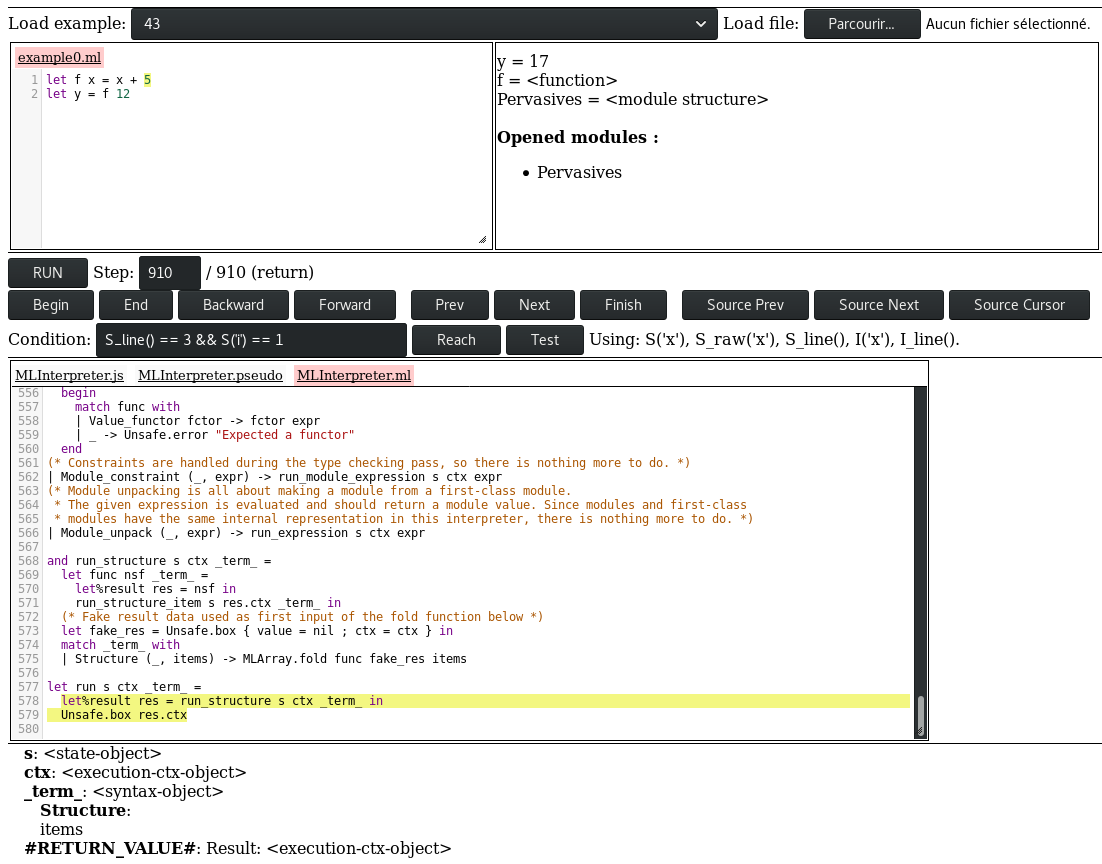
\includegraphics[width=\textwidth]{mlexplain}
\caption{MLExplain tournant dans l'interface de JSExplain}
\label{interface}
\end{figure}

\begin{figure}[hb]
\begin{tabular}[t]{| c | c |}
\hline
OCaml classique & OCaml reconnu par le compilateur de JSExplain \\
\hline
\begin{minipage}{0.40\textwidth}
\begin{lstlisting}
type num =
| Int of int
| Float of float

$(* Test d'égalité entre 2 num *)$
let eq a b = match (a, b) with
| (Int i1, Int i2) -> i1 = i2
| (Float f1, Float f2) -> f1 = f2
| (Int i, Float f) ->
  let fi = float_of_int i in
  fi = f
| (Float f, Int i) ->
  let fi = float_of_int i in
  fi = f
\end{lstlisting}
\end{minipage}
&
\begin{minipage}{0.47\textwidth}
\begin{lstlisting}
type num =
| Int of int [@f value]
| Float of float [@f value]

$(* Test d'égalité entre 2 num *)$
let eq a b = match a with
| Int i1 ->
  begin
    match b with
    | Int i2 -> i1 === i2
    | Float f2 ->
      let fi = float_of_int i1 in
      fi === f2
  end
| Float f1 ->
  begin
    match b with
    | Int i2 ->
      let fi = float_of_int i2 in
      fi === f1
    | Float f2 -> f1 === f2
  end
\end{lstlisting}
\end{minipage}
\\
\hline
\end{tabular}
\caption{Comparaison entre du code OCaml normal et son équivalent reconnu 
par JSExplain}
\label{code}
\end{figure}

\begin{figure}[hb]
\begin{lstlisting}
let js_of_case case =
  let js_patt = js_of_pattern case.patt in
  let js_guard = js_of_option js_of_expression case.guard in
  let js_expr = js_of_expression case.expr in
  Js.Unsafe.obj [|
    ("patt", js_patt) ;
    ("guard", js_guard) ;
    ("expr", js_expr) |]
\end{lstlisting}
\caption{Traduction du cas d'un filtrage de motif vers la 
représentation JavaScript de l'AST}
\label{js_of_case}
\end{figure}


\end{document}
